\documentclass{article}

% packages

\usepackage{graphicx}
\usepackage{cite}
\usepackage{url}
\usepackage{amsmath}

\begin{document}
\bibliographystyle{plain}

%title page
\pagenumbering{gobble}
\author{Joel Hill, Devon Haubold, Qammer Gul, Mohamed Bedru}
\title{Interception of Wireline Digital Signals Using Electromagnetic Fields}
\date{\today{}}
\maketitle{} %generate title

\newpage{}
\pagenumbering{roman}
\tableofcontents{}
\newpage
\pagenumbering{arabic}
\section{Introduction}
In a wired network, security is often focused on protecting the endpoints. Routers are kept behind lock and key, and when necessary ethernet ports are hidden or disconnected. The data itself can also be encrypted, a security layer that can be found in local network communication, as well as across the web. There are many cases however, where the encryption of data across a wired connection is not practical or is assumed to be unnecessary. The focus of this investigation was on these types of connections: unencrypted data sent from one computer to another over a wired connection.

Data can be sent over a physical connection using electric or optical signals. It has been shown that the data sent through fibre optic cable can be intercepted by bending the fibre optic cable enough for a small amount of light to escape. This escaped light can be read and parsed, thus allowing for undetected interception of data. 

An electric signal is not so easily intercepted without detection. It is possible to splice in and hardwire a connection, however this a time consuming process and may result in the detection of the third party. An ideal solution would be quick to implement, have little to no effect on the existing network, and portable. 

It has been hypothesized that wired electric signals can be intercepted by detecting the magnetic fields generated by the change in current as data is transferred.

\section{Fiber Optics Interception}
As wired signal transport methods shift from the traditional copper wire to optic fibre, security threats and vulnerabilities change. There was a time optic fibre was considered the most secure reliable means of network data transmission. This is not the case anymore as more advanced and cost effective methods of interception and intrusion are being developed. However, fibre optics is still the preferred method of transporting big data due to two reasons: Fibre transports large volumes of data very fast and can transport data for long distances with little loss. Law enforcement Agencies, Intelligence agencies, Defense, Telecom Service Providers and Cyber Security are already using devices which can tap optic fibre cables to select, extract and monitor data. One example is the recent leak which shows how the NSA taps an undersea cable \cite{atlantic}. It is worse when information is accessed by criminals or those who want to inflict harm on us. It has been proven that a very cheap clip-on coupler can be used by individuals to easily tap a fibre \cite{opterna}

\subsection{Vulnerabilities}
Optic fibre data transmission used to be considered secure as it was difficult to intercept the transmission without detection. The methods and devices used to tap into optical fibre were very expensive and as such, it was not easy or realistic for an ordinary person to intercept a transmission. Technology has now advanced to the point where fibre optic interception has become inexpensive and easily available. Some of the vulnerabilities and methods used to tap into fibre are explained below:

\subsubsection{Curving}
It is possible to make a detectable amount of light to leak from optical fibre through bending. With the proper equipment, the data in the leaked light can be captured with only a small leak. This method works well at low data rates but is less effective with as rates increase. \cite{sans} 

\subsubsection{Splicing}
To tap into the cable using this method, a device is used to make a break in the cable and the data is then monitored. Splicing stops data transmission for very short time which might make detection possible. However, most cables already have splice point for maintenance purpose and those points can easily be manipulated. This tapping works only for a short period of time and is not preferred. \cite{sans}

\subsubsection{Protecting Optical Data Transimission}
Even if nothing can be fully secure, it is possible to stop intrusion or minimize the risk. The best way to stop this kind of data theft is by using strong encryption to make the stolen data useless. Once the data reaches the receiver, the encrypted data will be converted to meaningful data. 

\section{Interception of Electrical Signals}

Faraday's law states that a closed circuit can be acted upon by an electromagnetic force if the surrounding magnetic field undergoes a change in state. Changes in the position of the circuit relative to the field, the intensity of the field, or the orientation of the circuit relative to the field will all generate an EMF that acts on the circuit. \cite{faraday}

If the closed circuit within the magnetic field happens to be a wire coil, the EMF induced on the coil with produce a voltage difference within the coil as described in the following equation:

\begin{equation*}
 V = -N(\Delta B A)/\Delta t
 \end{equation*}
 
Where $V$ is voltage, $N$ is the number of coils in the circuit, $\Delta B A$ is the change in the magnetic field, and $\Delta t$ is the change in time.
 
It is also known that current traveling in a straight line through a wire with produce a perpendicular magnetic field around the wire. Since data sent via a wired transmission is represented by high and low voltage states, it is also the case that a wired transmission of data will produce a magnetic flux in the area around the wire that is also representative of the data \cite{magneticfields}.
 
It is hypothesized that a closed circuit can be designed that will take advantage of Faraday's law and detect the changing magnetic fields around a wired data transmission. This hypothetical device could then allow a user to parse the voltage changes into binary data and intercept the wired transmission without physically altering the wire in any way.

\subsection{Experiments and Methods}
Several experiments were conducted in order to test the practicality of wirelessly intercepting a wired transmission via magnetic fields.

\subsubsection{Intercepting Analog Data}
A wire coil approximately 1cm in diameter was built using magnet wire (very thinly coated wired designed for electric motor or speaker construction). The coil had approximately 50 - 60 wire loops. Each end of the wire coil was attached to a terminal on a headphone jack.

\begin{figure}
	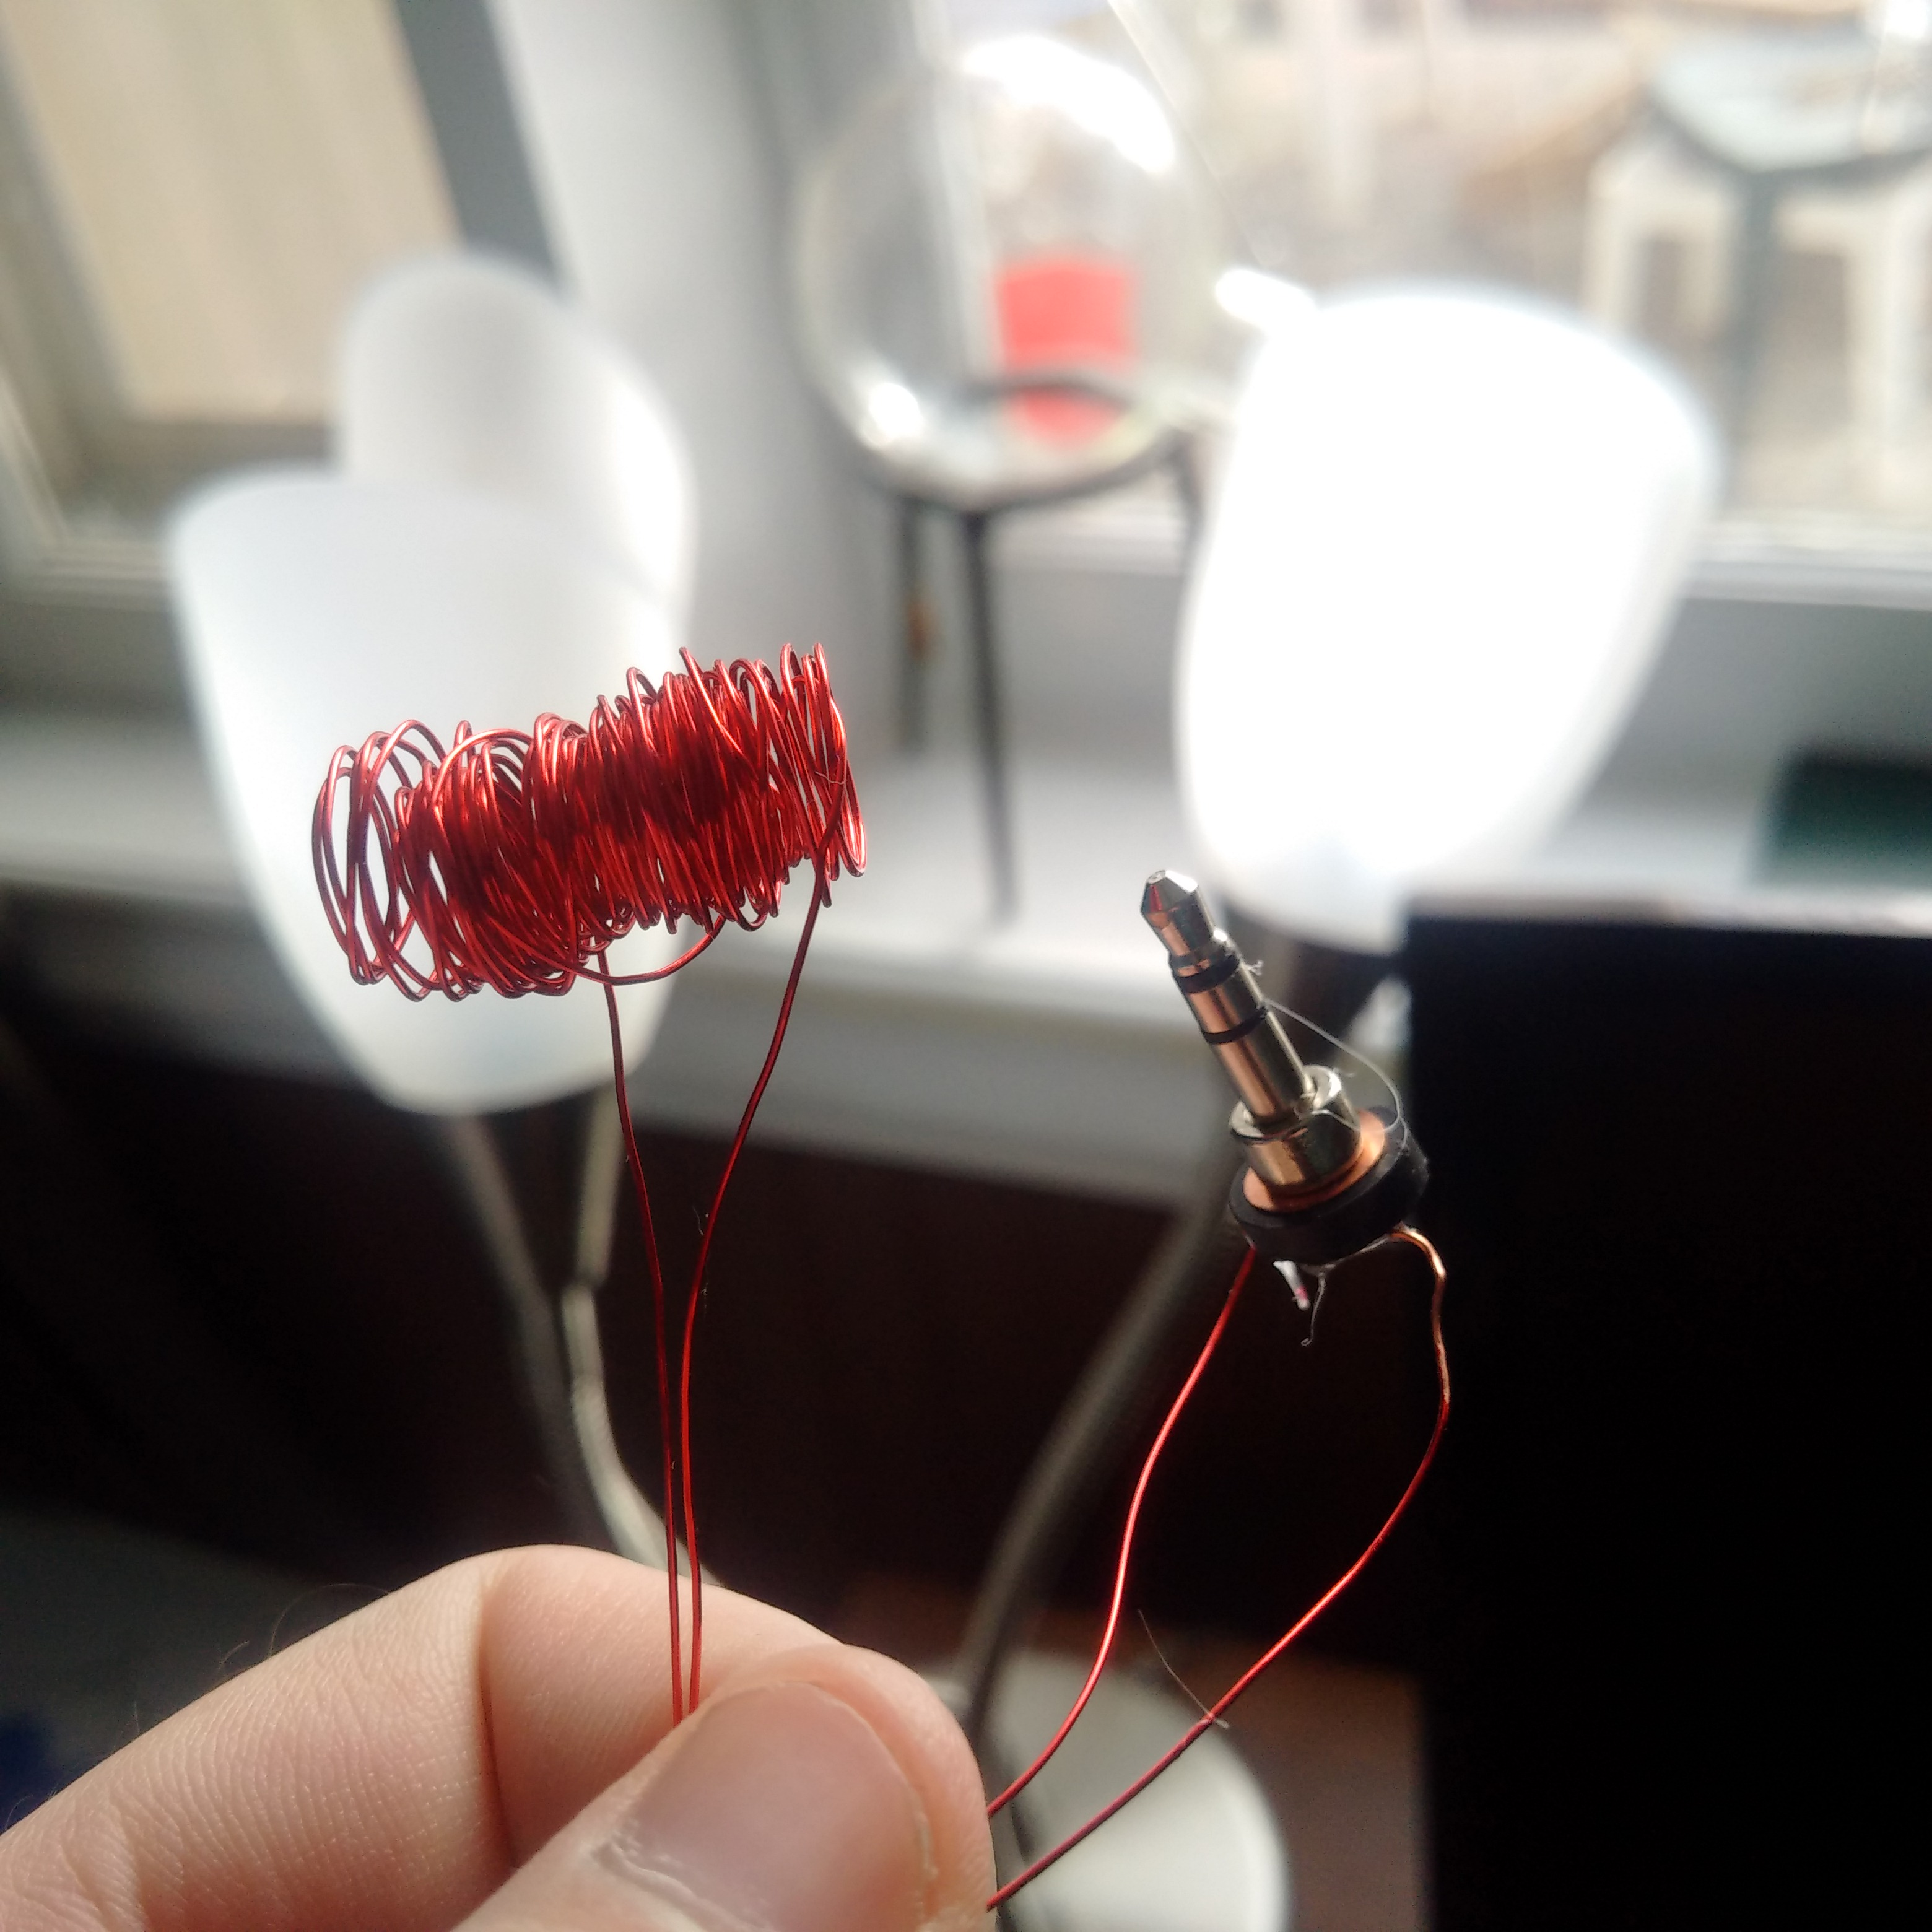
\includegraphics[width=\linewidth]{images/coil_jack.jpg}
	\caption{Wire coil connected to audio jack.}
	\label{fig:coil_jack}
\end{figure}

It was hypothesized that by surrounding an audio cable with the wire coil as an audio signal was transmitted, current would be generated in the coil. If the attached headphone jack were to be inserted into recording equipment, the generated current could be interpreted as sound and could be recorded with audio processing software.

An experiment was conducted where music was played from a receiver to a set of external speakers via a standard audio cable. The wire coil was placed around the audio cable and plugged into an audio input jack on a nearby computer. As the music played, the voltage from the wire coil was recorded.

It was observed that current was indeed produced in the wire coil due to the audio transmitted through the cable. The resulting signal however did not resemble the original data being sent. Based on Faraday's law this was expected, since only changes in magnetic fields produce voltage in the coil, not constant values. This means the analog signal produces a corresponding but different signal in the coil.

\subsubsection{Intercepting Digital Data Sent From Raspberry Pi Computer}

Raspberry Pis are single board Linux computers with built in General Purpose Input/Output(GPIO) pins. It was determined that a custom data transfer protocol could be written that would use the GPIO pins to send data from one Raspberry Pi computer to another. This would allow for ideal conditions in which the interception of data via magnetic fields could be tested since the data would be send over a single wire, the frequency of the data could be controlled, and the Voltage/Current was a known value.

A custom data protocol was written in Python. The data was transferred by converting short strings of text into binary numbers representing the ASCII values of the individual characters. Each message was also preceded by a start character, and terminated by a predetermined end character. Two separate scripts were used: one to parse and send the message, and the other to listen and receive the message. In both cases, each program was hard-coded to use a constant frequency, and to use voltage changes in the GPIO pins as representations of 1\textquoteright s and\textquoteright s.

Tests were conducted on the protocol, and it was concluded that the method worked when sending short strings of characters from one Raspberry Pi computer to another. The wire coil from the previous experiment was then wrapped around the transmission wire and plugged into a laptop. As done in the analog signal test, the audio from the wire coil was recorded as messages were sent.

It was observed that the downward and upward edges in the wire-line transmission could be detected by the wire coil at various frequencies, although the data  was near impossible to parse without computer assistance. The results from sending an unending string of ones and zeros at various frequencies is illustrated in the following figures 2 and 3.

\begin{figure}
	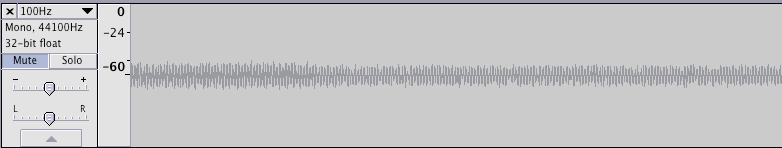
\includegraphics[width=\linewidth]{images/100hz.png}
	\caption{Data transmitted at 100Hz intercepted by wire coil.}
	\label{fig:100hz}
\end{figure}

\begin{figure}
	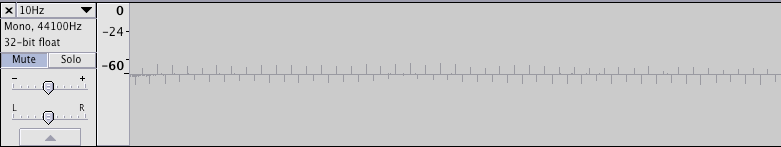
\includegraphics[width=\linewidth]{images/10hz.png}
	\caption{Data transmitted at 10Hz intercepted by wire coil.}
	\label{fig:10hz}
\end{figure}

After confirming that the data send via wire-line from one Raspberry Pi to another could be detected by a wire coil, and attempt was made to have a third computer interpret the data and parse the message.

A single Raspberry Pi was reconfigured to send a message to itself by directly wiring an output pin to an input pin. The second raspberry pin was connected to a wire coil that was wrapped around the data transmission line. Attempts were made to intercept the message as it was transmitted through the data cable. It was observed that the wire coil was not producing enough voltage to be detected by the GPIO pins, and so a different approach was needed.

\subsubsection{Intercepting Digital Signal Sent From Square Wave Generator}

The Raspberry Pi experiments demonstrated that the wire coil was capable of responding to a wire-line transmission of data, but a precise correlation between high and low voltage edges in the data transmission and the signal generated from the wire coil was not observed.

Rather than using a Raspberry Pi computer, a square wave generator was used to simulate a digital data signal. It was theorized that a square wave generator could transmit data at a higher power level, thus producing a stronger magnetic field. The generator was set to produce a wave with amplitude of 5V at a frequency of 100Hz. This simulates a bit rate of 0.1Kb/s.

A new wire coil was also built, this time with a much smaller diameter, more precise coil placement, and approximately 100 coils. It was hypothesized that the new coil would be more sensitive and produce less noise. The circuit diagram of the experiment is illustrated in figure 4, while figure 5 depicts the experiment as it was built in the lab.

\begin{figure}
	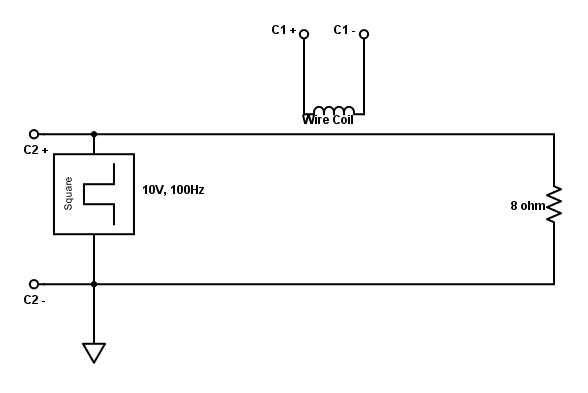
\includegraphics[width=\linewidth]{images/circuit_diagram.png}
	\caption{Circuit diagram of square wave generator experiment.}
	\label{fig:square}
\end{figure}

\begin{figure}
	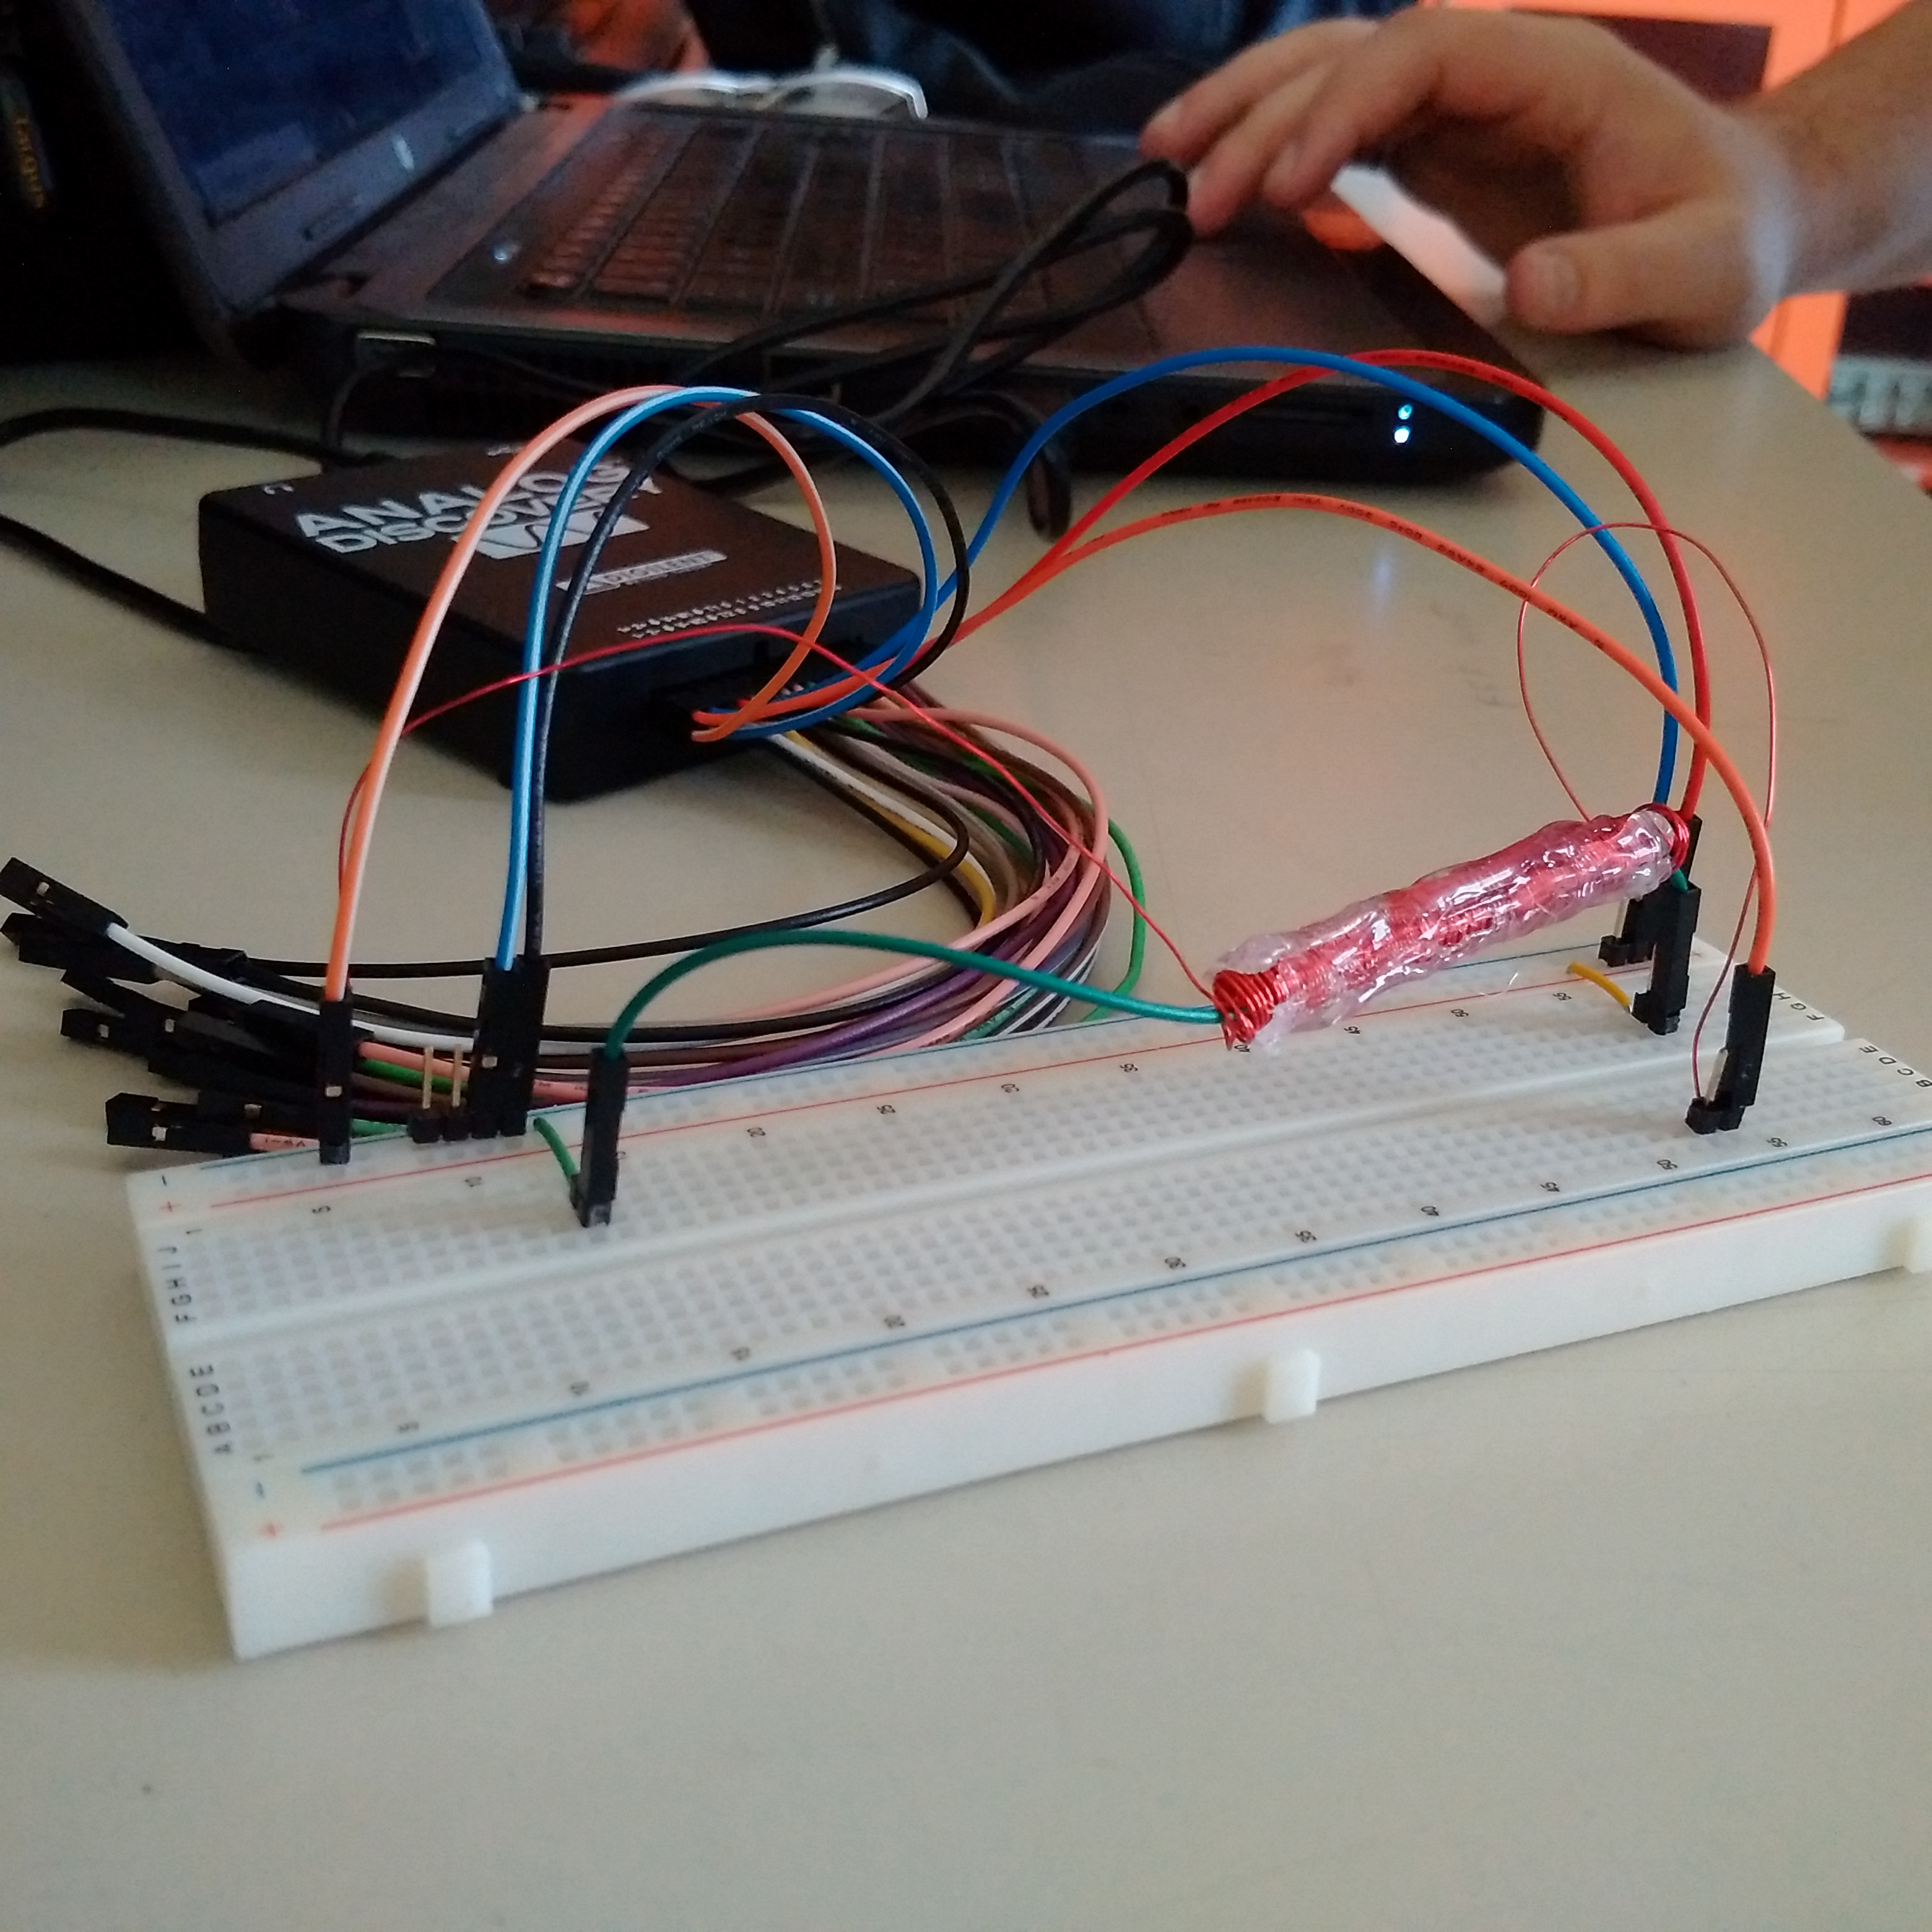
\includegraphics[width=\linewidth]{images/circuit.jpg}
	\caption{Depiction of square wave generator experiment.}
	\label{fig:squarepic}
\end{figure}

A stream of alternating high and low voltages representing 1s and 0s was generated, and the signal was monitored by a digital oscilloscope. The wire coil was also monitored by the digital oscilloscope, and the resulting voltages from both channels was recorded. 

\begin{figure}
	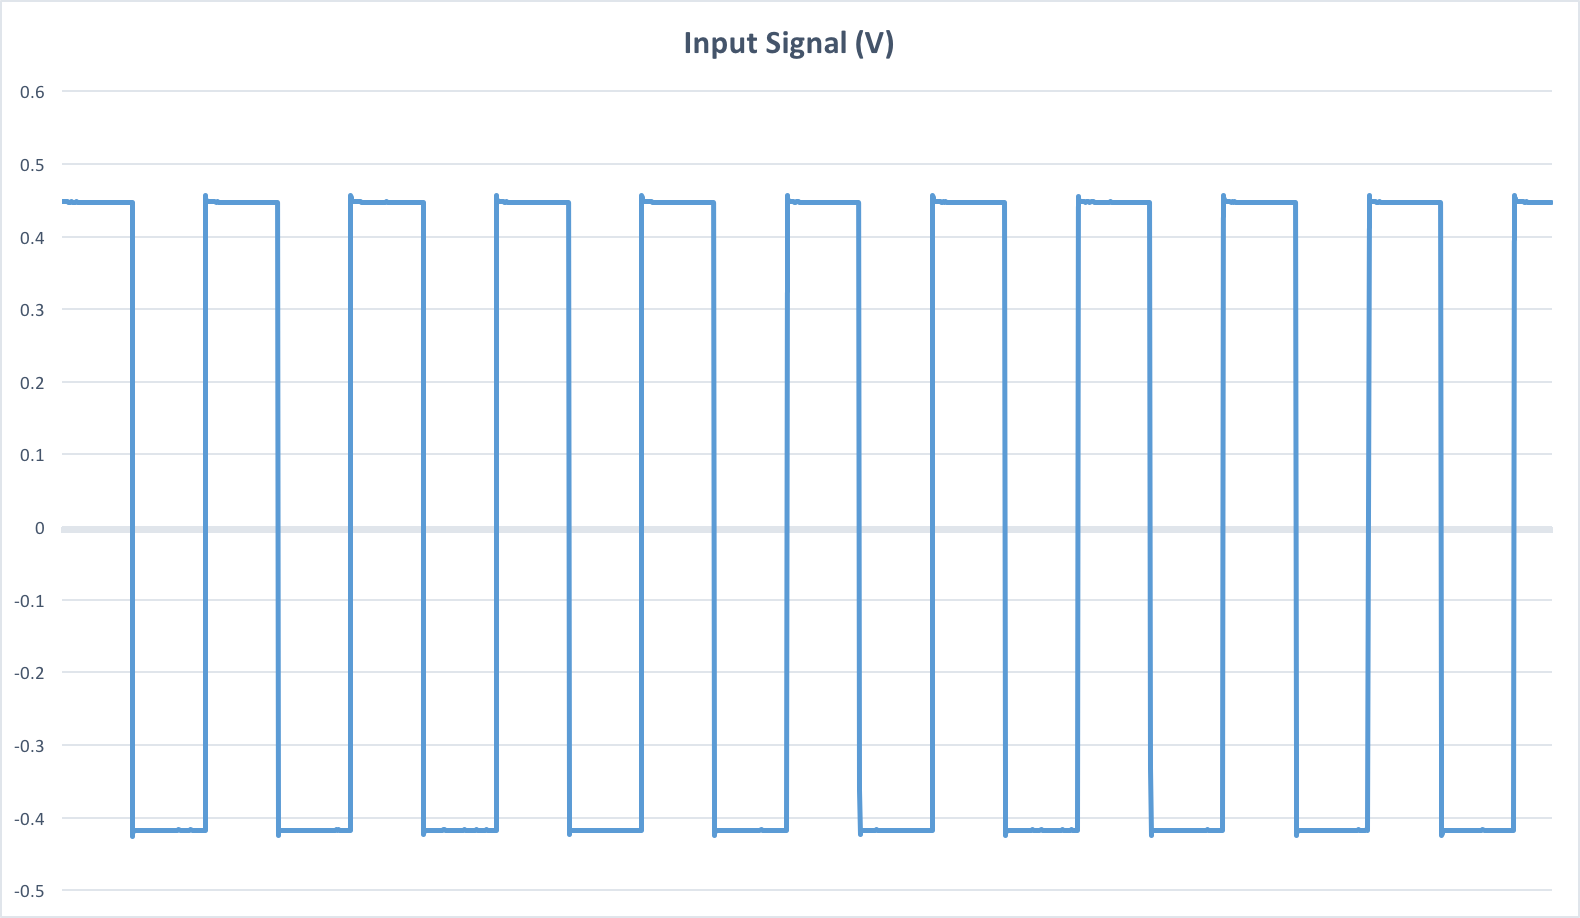
\includegraphics[width=\linewidth]{images/input.png}
	\caption{Generated square wave.}
	\label{fig:square_wave}
\end{figure}

\begin{figure}
	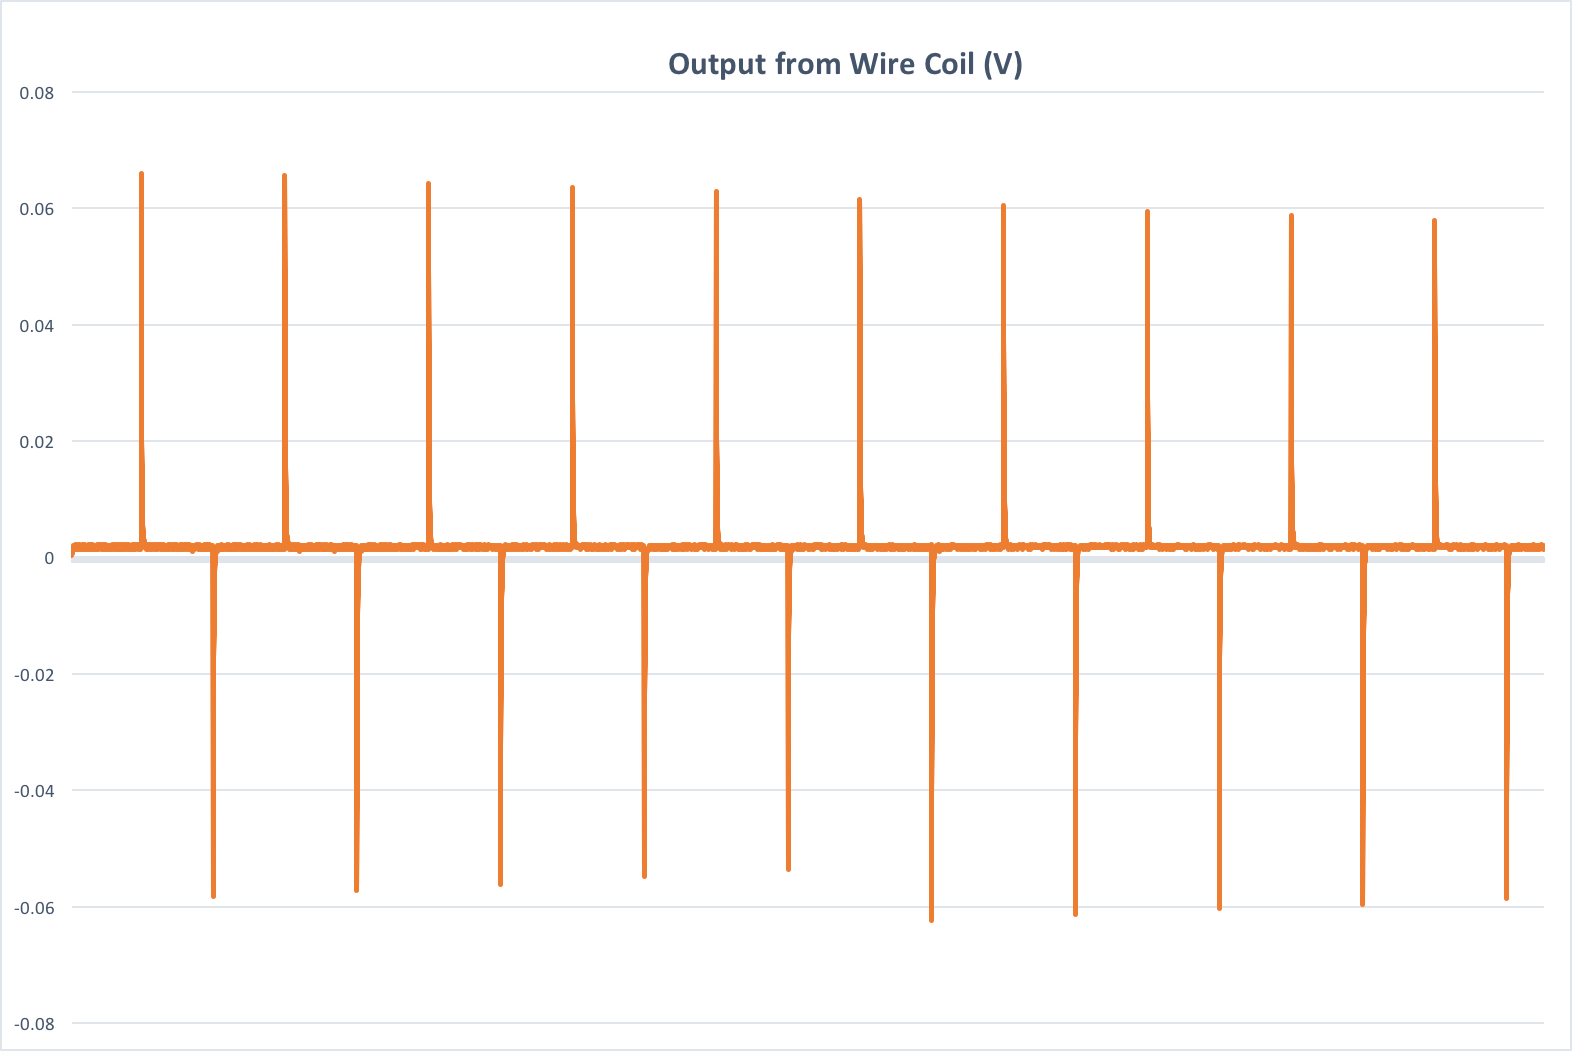
\includegraphics[width=\linewidth]{images/coil.png}
	\caption{Voltage detected in wire coil.}
	\label{fig:output}
\end{figure}

\begin{figure}
	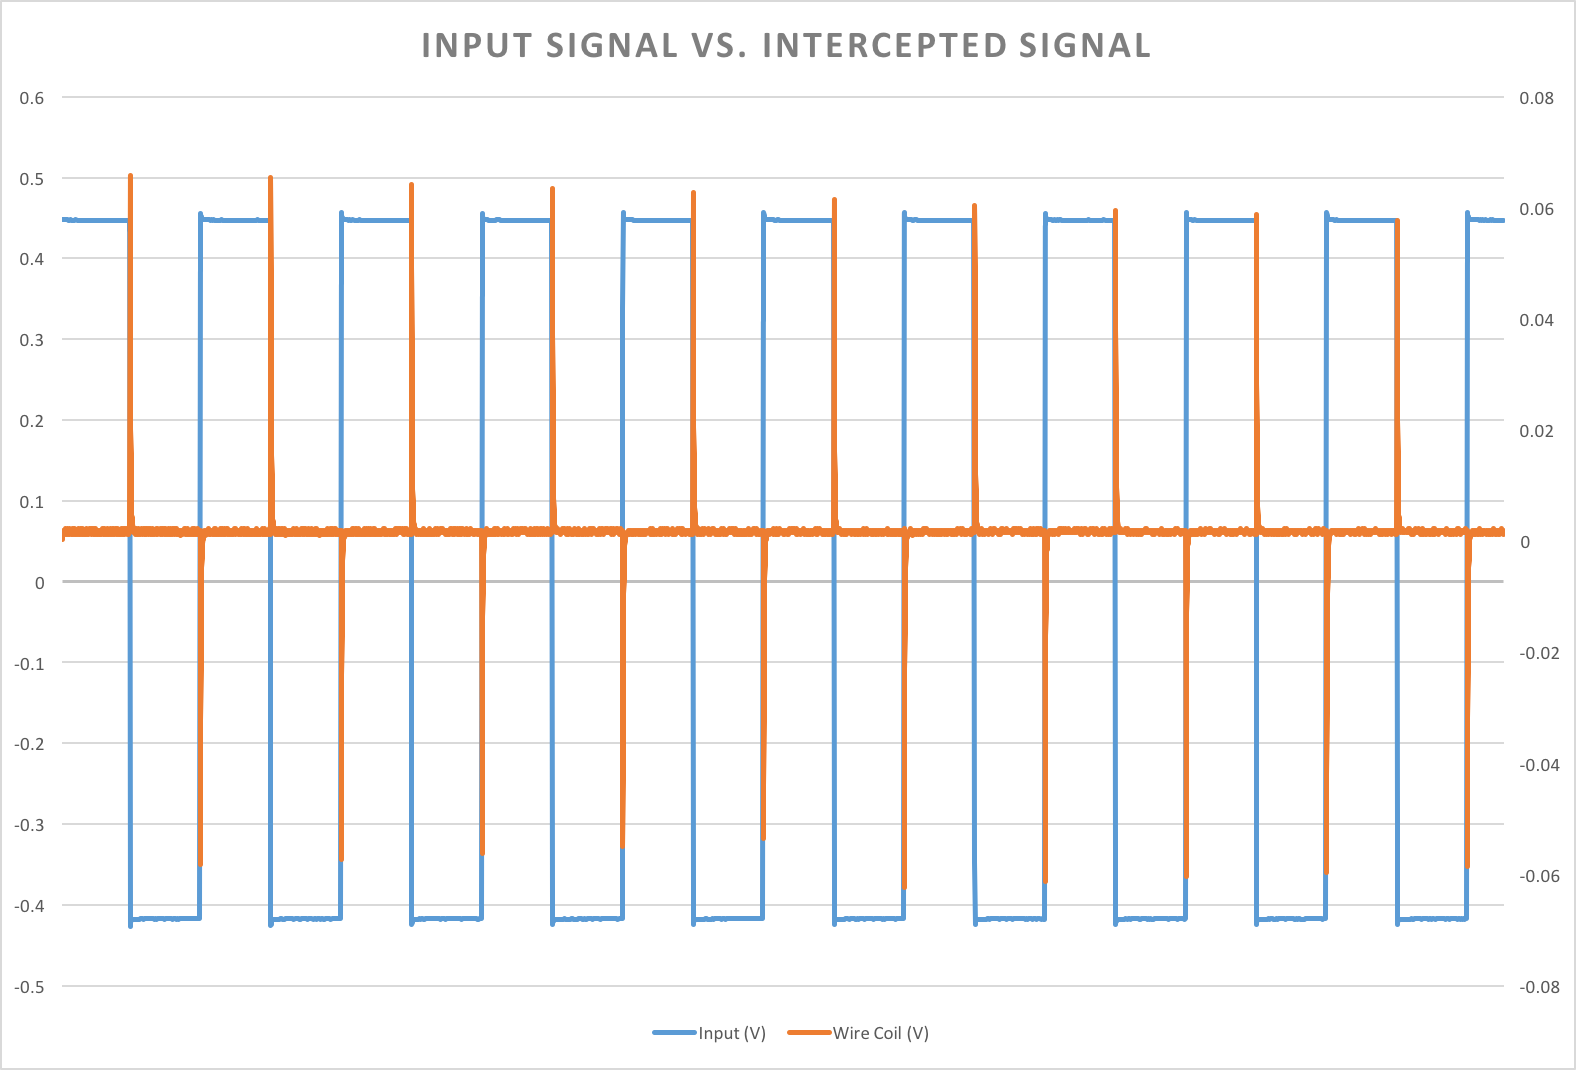
\includegraphics[width=\linewidth]{images/combined.png}
	\caption{Input square wave overlaid with wire coil output.}
	\label{fig:combined}
\end{figure}

Figures 6, 7, and 8 depict the results obtained from the experiments. Figure 6 illustrates a consistent square wave representing alternating 1s and 0s in a binary transmission. Figure 7 illustrates the alternating voltage spikes in voltage detected in the wire coil wrapped around the transmission line. Figure 8 illustrates the direct correlation between upward and downward edges in the data transmission with the positive and negative spikes in voltage observed in the wire coil.

\section{Conclusions}

The research and experiments conducted indicate that wired data transmissions are vulnerable to interception. fibre optic cables are susceptible to techniques that splice the cable, as well as less invasive methods involving the detection of minute levels of escaping light from the cable.

Information transmitted via electric cable is also vulnerable to wireless interception. The experiments conducted and outlined in this paper indicate that the wired transmission of data produces minute magnetic fields that can be detected and parsed by sophisticated equipment. Although none of the experiments emulated real life conditions where this type of security breach can occur, they did demonstrate that the technique is at least possible given the right combination of hardware and software.

\newpage{}
\bibliography{references}
\end{document}
